\documentclass[12pt,a4paper,UTF8]{article}

\usepackage[titletoc]{appendix}
\usepackage{xeCJK}
\usepackage{amsmath}
\usepackage{array}
\usepackage{bm}
\usepackage{booktabs}
\usepackage{caption}
\usepackage{cite}
\usepackage{comment}
\usepackage{float}
\usepackage{fontspec} % xelatex限定
\usepackage{geometry}
\usepackage{graphicx}
\usepackage{indentfirst}
% \usepackage[utf8]{inputenc} % 非xelatex编译,显式指定文件编码为utf8
\usepackage{listings}
\usepackage{longtable}
\usepackage{mathtools}
\usepackage{multicol}
\usepackage{multirow}
\usepackage{supertabular}
\usepackage{subcaption}
\usepackage{tabu}
\usepackage{ulem}
\usepackage{url}
\usepackage{xcolor}
\usepackage{nccmath} % だが align* は nccmath が無くても使えるので敢えて両方書いた。
% \usepackage{CJKutf8}
% \usepackage{hyperref}

\geometry{a4paper,left=2.5cm,right=2.5cm,top=2.5cm,bottom=2.5cm}
\defaultCJKfontfeatures{Scale=1.2}
\linespread{1.5}

%% Define a new 'leo' style for the package that will use a smaller font.
\makeatletter
\def\url@leostyle{%
  \@ifundefined{selectfont}{\def\UrlFont{\sf}}{\def\UrlFont{\small\ttfamily}}}
\makeatother
\urlstyle{leo} % Now actually use the newly defined style.


\renewcommand{\contentsname}{\centering{目录}}
\renewcommand{\abstractname}{\large{摘要}}
\def\tablename{表}
\def\figurename{图}
\renewcommand{\thetable}{\thesection.\arabic{table}}
\renewcommand{\thefigure}{\thesection.\arabic{figure}}
\renewcommand{\multirowsetup}{\centering}
\renewcommand{\appendixname}{附录~\Alpha{section}}
\renewcommand{\refname}{参考文献}

\everymath{\displaystyle}
\bibliographystyle{plain}


\lstdefinestyle{BASH}{
    breaklines=true,                                     % 自动换行
    columns=fixed,
    extendedchars=true,                                  % lets you use non-ASCII characters; for 8-bits encodings only, does not work with UTF-8
    frame=shadowbox,                                     % 设置背景边框
    numbers=left,                                        % 在左侧显示行号
    numberstyle=\footnotesize\color{darkgray},           % 设定行号格式
    showstringspaces=false,                              % 不显示字符串中的空格
    tabsize=4,	                                         % 设置tab长度
}
\lstdefinestyle{tinyBASH}{
    breaklines=true,                                     % 自动换行
    basicstyle=\footnotesize\ttfamily,
    columns=fixed,
    extendedchars=true,                                  % lets you use non-ASCII characters; for 8-bits encodings only, does not work with UTF-8
    frame=shadowbox,                                     % 设置背景边框
    numbers=left,                                        % 在左侧显示行号
    numberstyle=\footnotesize\color{darkgray},           % 设定行号格式
    showstringspaces=false,                              % 不显示字符串中的空格
    tabsize=4,	                                         % 设置tab长度
}
\lstdefinestyle{Python}{
    breaklines=true,                                     % 自动换行
    captionpos=b,                                        % sets the caption-position to bottom
    columns=fixed,
    commentstyle=\it\color[RGB]{0,96,96},                % 设置代码注释的格式
    % extendedchars=true,                                  % lets you use non-ASCII characters; for 8-bits encodings only, does not work with UTF-8
    frame=shadowbox,                                     % 设置背景边框
    keywordstyle=\bfseries\color[RGB]{40,40,255},        % 设定关键字颜色
    language=Python,                                     % 设置语言
    numbers=left,                                        % 在左侧显示行号
    numberstyle=\footnotesize\color{darkgray},           % 设定行号格式
    stringstyle=\rmfamily\slshape\color[RGB]{128,0,0},   % 设置字符串格式
    tabsize=4,	                                         % 设置tab长度
}

\lstdefinestyle{CPP}{
    %backgroundcolor=\color[RGB]{245,245,244},           % 设定背景颜色
    breaklines=true,                                     % 自动换行
    captionpos=b,                                        % sets the caption-position to bottom
    columns=fixed,
    commentstyle=\it\color[RGB]{0,96,96},                % 设置代码注释的格式
    extendedchars=true,                                  % lets you use non-ASCII characters; for 8-bits encodings only, does not work with UTF-8
    frame=shadowbox,                                     % 设置背景边框
    keywordstyle=\bfseries\color[RGB]{40,40,255},        % 设定关键字颜色
    language=c++,                                        % 设置语言
    numbers=left,                                        % 在左侧显示行号
    numberstyle=\footnotesize\color{darkgray},           % 设定行号格式
    showstringspaces=false,                              % 不显示字符串中的空格
    stringstyle=\rmfamily\slshape\color[RGB]{128,0,0},   % 设置字符串格式
    tabsize=4,	                                         % 设置tab长度
    title=\lstname,                                      % show the filename of files included with \lstinputlisting; also try caption instead of title
    morekeywords={alignas,continute,friend,register,true,alignof,decltype,goto,
        reinterpret_cast,try,asm,defult,if,return,typedef,auto,delete,inline,short,
        typeid,bool,do,int,signed,typename,break,double,long,sizeof,union,case,
        dynamic_cast,mutable,static,unsigned,catch,else,namespace,static_assert,using,
        char,enum,new,static_cast,virtual,char16_t,char32_t,explict,noexcept,struct,
        void,export,nullptr,switch,volatile,class,extern,operator,template,wchar_t,
        const,false,private,this,while,constexpr,float,protected,thread_local,
        const_cast,for,public,throw,std},
    emph={map,set,multimap,multiset,unordered_map,unordered_set,
        unordered_multiset,unordered_multimap,vector,string,list,deque,
        array,stack,forwared_list,iostream,memory,shared_ptr,unique_ptr,
        random,bitset,ostream,istream,cout,cin,endl,move,default_random_engine,
        uniform_int_distribution,iterator,algorithm,functional,bing,numeric},
}

\lstdefinestyle{QT}{
    %backgroundcolor=\color[RGB]{245,245,244},           % 设定背景颜色
    breaklines=true,                                     % 自动换行
    captionpos=b,                                        % sets the caption-position to bottom
    columns=fixed,
    commentstyle=\it\color[RGB]{0,96,96},                % 设置代码注释的格式
    extendedchars=true,                                  % lets you use non-ASCII characters; for 8-bits encodings only, does not work with UTF-8
    frame=shadowbox,                                     % 设置背景边框
    keywordstyle=\bfseries\color[RGB]{40,40,255},        % 设定关键字颜色
    language=c++,                                        % 设置语言
    numbers=left,                                        % 在左侧显示行号
    numberstyle=\footnotesize\color{darkgray},           % 设定行号格式
    stringstyle=\rmfamily\slshape\color[RGB]{128,0,0},   % 设置字符串格式
    showstringspaces=false,                              % 不显示字符串中的空格
    tabsize=4,	                                         % 设置tab长度
    title=\lstname,                                      % show the filename of files included with \lstinputlisting; also try caption instead of title
    morekeywords={alignas,continute,friend,register,true,alignof,decltype,goto,
        reinterpret_cast,try,asm,defult,if,return,typedef,auto,delete,inline,short,
        typeid,bool,do,int,signed,typename,break,double,long,sizeof,union,case,
        dynamic_cast,mutable,static,unsigned,catch,else,namespace,static_assert,using,
        char,enum,new,static_cast,virtual,char16_t,char32_t,explict,noexcept,struct,
        void,export,nullptr,switch,volatile,class,extern,operator,template,wchar_t,
        const,false,private,this,while,constexpr,float,protected,thread_local,
        const_cast,for,public,throw,std,bind,function,
        Q_OBJECT,QDialog,QUdpSocket,QTcpSocket,QHostAddress,QNetworkDatagram,QTcpServer,
        QByteArray,QString,QStringList,QList,QSet,QMap,
        quint,qint64,uintptr_t,
        connect,signals,slots,SIGNAL,SLOT},
    emph={map,set,multimap,multiset,unordered_map,unordered_set,
        unordered_multiset,unordered_multimap,vector,string,list,deque,
        array,stack,forwared_list,iostream,memory,shared_ptr,unique_ptr,
        random,bitset,ostream,istream,cout,cin,endl,move,default_random_engine,
        uniform_int_distribution,iterator,algorithm,functional,bing,numeric},
}

\lstdefinestyle{MASM}{
    breaklines=true,                                     % 自动换行
    captionpos=b,                                        % sets the caption-position to bottom
    columns=fixed,
    commentstyle=\it\color[RGB]{0,96,96},                % 设置代码注释的格式
    extendedchars=true,                                  % lets you use non-ASCII characters; for 8-bits encodings only, does not work with UTF-8    
    frame=shadowbox,                                     % 设置背景边框
    keywordstyle=\bfseries\color[RGB]{40,40,255},        % 设定关键字颜色
    language=[x86masm]Assembler,                         % 设置语言
    numbers=left,                                        % 在左侧显示行号
    numberstyle=\footnotesize\color{darkgray},           % 设定行号格式
    stringstyle=\rmfamily\slshape\color[RGB]{128,0,0},   % 设置字符串格式
    showstringspaces=false,                              % 不显示字符串中的空格
    tabsize=4,	                                         % 设置tab长度
    title=\lstname,                                      % show the filename of files included with \lstinputlisting; also try caption instead of title
    morekeywords={CDQE,CQO,CMPSQ,CMPXCHG16B,JRCXZ,LODSQ,MOVSXD, % 
        POPFQ,PUSHFQ,SCASQ,STOSQ,IRETQ,RDTSCP,SWAPGS, % 
        .code,.def,.file,.type,.ended,.scl,.section,.ascii,.text,.globl,.ident,.rodata,
        .sch_proc,.sch_pushreg,.sch_setframe,.sch_stackalloc,.sch_endprologue,.sch_endproc,
        pushq,popq,movq,movl,addq,subq,leaq,invoke,start,addr,
        rax,rdx,rcx,rbx,rsi,rdi,rip,rsp,rbp, % 
        r8,r8d,r8w,r8b,r9,r9d,r9w,r9b, % 
        r10,r10d,r10w,r10b,r11,r11d,r11w,r11b, % 
        r12,r12d,r12w,r12b,r13,r13d,r13w,r13b, % 
        r14,r14d,r14w,r14b,r15,r15d,r15w,r15b}
}
\newcommand{\includecode}[2][c]{\lstinputlisting[caption=#2, escapechar=, style=#1]{#2}}



% \setcounter{table}{0}
% \setcounter{figure}{0}

% \lstinputlisting[style=CPP]{src/main.cpp}

% \begin{figure}[H]
%     \centering
%     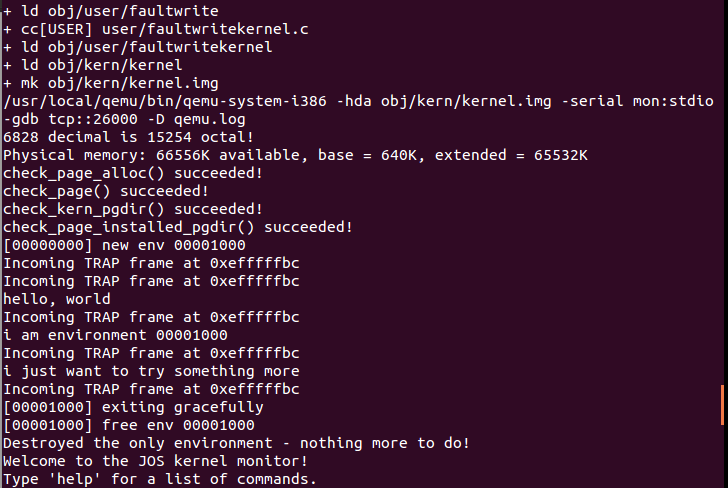
\includegraphics[width = .75\linewidth]{img/1.png}
%     \caption{预处理结果(部分)}
%     \label{fig::figure2}
% \end{figure}


% 结果如表\ref{tab::table2}:
% \begin{table}[htbp]
%     \begin{center}
%         \begin{tabular}{c c c}
%             \toprule
%             优化等级 & 二进制文件大小(Byte) &  执行时间(s)\\
%             \midrule
%             不优化 & 13992 & 36.090 \\
%             O1 & 13344 & 10.562\\
%             O2 & 13344 & 9.925\\
%             Os & 13344 & 8.899\\
%             O3 & 13344 & 8.350\\
%             Ofast & 14800 & 8.094\\
%             \bottomrule
%         \end{tabular}
%         \caption{各等级优化测试结果}\label{tab::table2}
%     \end{center}
% \end{table}

% \begin{equation}
%     \begin{split}
%         id     & \rightarrow char\ |\ id\ digit\ |\ id\ char \\
%         digit  & \rightarrow 0\ |\ 1\ |\ 2\ |\ 3\ |\ 4\ |\ 5\ |\ 6\ |\ 7\ |\ 8\ |\ 9 \\
%         char   & \rightarrow \_\ |\ letter \\
%         letter & \rightarrow A\ |\ B\ |\ ...\ |\ Z\ |\ a\ |\ b\ |\ ...\ |\ z \\
%     \end{split}
% \end{equation}


\begin{document}

\title{Lab 3:  User Environment}
\author{\ }
\date{\today}

\maketitle

\begin{abstract}
    \setlength{\parindent}{2em}
    本次实验取自MIT\ 6.828\ Lab3,共分为两个部分。第一部分为用户环境与异常处理。第二部分为缺页中断、断点异常和系统调用。
    在本次实验中,将实现使保护模式下的用户进程得以运行的基础内核功能,并对JOS 内核建立用于追踪用户进程的数据结构,
    创建用户进程,读入程序映像并运行。同时,要使JOS 内核有能力响应用户进程的任何系统调用,并处理用户进程所造成的异常。

    \textbf{关键词:JOS、用户环境、中断、异常、系统调用}
\end{abstract}

\section{作业一}
    \subsection{全局变量}
    kern/env.c中定义的三个全局变量envs、curenv、env\_free\_list分别表示所有进程、当前正在运行的进程和空闲进程链表。

    JOS启动并开始运行,envs指针便指向了一个 Env 结构体链表,表示系统中所有的用户环境的env。JOS内核把所有不活跃的Env结构体,
    用env\_free\_list链接起来,方便进行用户环境env的分配和回收。内核也会把 curenv 指针指向在任意时刻正在执行的用户环境的 Env 结构体。
    在内核启动时,并且还没有任何用户环境运行时,curenv的值为NULL。


    \subsection{ENV结构体}
    inc/env 中定义了 Env 结构体,各部分功能如下:

    \begin{lstlisting}[style=CPP]
struct Env
{
    struct Trapframe env_tf;
    struct Env *env_link;
    envid_t env_id;
    envid_t env_parent_id;
    enum EnvType env_type;
    unsigned env_status;
    uint32_t env_runs;

    pde_t *env_pgdir;
};
    \end{lstlisting}

    env\_tf:
    存储当进程没有在运行时被保存下来的寄存器的值。
    具体来说,当内核或者另一个不同的进程在运行的时候。内核在从用户模式切换到内核模式时将上一个进程的寄存器的值保存下来,
    从而进程可以从它被暂停的时间点恢复过来。
    
    env\_link:
    指向下一个位于 env\_free\_list 中的 Env 结构体的指针。env\_free\_list 指向链表中第一个空闲进程。
    
    env\_id:
    存储可以唯一确定正在使用这个 Env 数组的进程标识符。
    
    env\_parent\_id:
    存储创建这个进程的 env\_id。通过这种方式,进程可以形成一个 进程树 (family\ tree),
    可用于在做一些安全决定时来确定某个进程能对哪些进程所执行的动作。
    
    env\_type:
    用来区别一些特殊的进程。对于大多数进程,它会是 ENV\_TYPE\_USER。
    也可引入一些其他类型,来表示特殊的系统服务进程。
    
    env\_status:
    这个变量的值可能是下面这些中的一个:

    ENV\_FREE: 这个 Env 结构未被利用,因此在 env\_free\_list 中。

    ENV\_RUNNABLE: 表示一个正在等待进入处理器运行的进程。

    ENV\_RUNNING: 表示目前正在运行的进程。

    ENV\_NOT\_RUNNABLE: 表示目前已经激活的进程,但是它还没有准备好运行,例如,
    它可能在等其他进程的进程间通信(interprocess communication, IPC)。

    ENV\_DYING: 表示一个僵尸进程。僵尸进程将在下一次陷入内核的时候被释放。
    
    env\_pgdir:
    储存这个进程的页目录的内核虚拟地址
   
    \subsection{作业一实现}
    作业1要求修改 kern/pmap.c 中的 mem\_init() 函数来分配并映射envs数组。则对函数进行修改,
    首先要在page\_init()之前对envs进行初始化并分配内存空间。
    然后要在check\_page()函数之后的页表中设置它的映射关系。程序如下修改内容所示:
    
    \begin{lstlisting}[style=CPP]
envs = (struct Env*)boot_alloc(NENV*sizeof(struct Env));
memset(envs, 0, NENV*sizeof(struct Env));
boot_map_region(kern_pgdir, UENVS, PTSIZE, PADDR(envs), PTE_U);
    \end{lstlisting}

    make qemu时发现boot\_map\_region 函数中在for循环里定义变量类型,可以通过gcc src.c -std=c99 -o src 
    将GCC换成C99标准或者将变量类型在for循环外面定义,从而可以看到check\_kern\_pgdir() succeeded!

\section{作业二}
    \subsection{作业要求}
    在 env.c 中,完成以下函数

    env\_init() 初始化全部 envs 数组中的 Env 结构体,并将它们加入到 空闲进程链表env\_free\_list 中。

    env\_setup\_vm() 为新的进程分配一个页目录,并初始化新进程的地址空间对应的内核部分。

    region\_alloc() 为进程分配和映射物理内存。

    load\_icode() 处理 ELF 二进制映像,并将映像内容读入新进程的用户地址空间。

    env\_create() 通过调用 env\_alloc 分配一个新进程,并调用 load\_icode读入 ELF 二进制映像。

    env\_run() 启动给定的在用户模式运行的进程。

    \subsection{env\_init()}

    遍历envs数组中的所有Env结构体,把每一个结构体的 env\_id 字段置0,并将它们插入到env\_free\_list中。
    envs中的env\_link指向的是下一个env,为确保环境在空闲列表中的顺序与它们在envs数组中的顺序相同,
    也就是envs[0]在链表头部位置,插入时从后往前插入。

    插入结束后调用env\_init\_percpu 通过配置段硬件将其分隔为特权等级 0 (内核) 和特权等级 3(用户)两个不同的段。

    \begin{lstlisting}[style=CPP]
void
env_init(void)
{
    // Set up envs array
    // LAB 3: Your code here.
    int i=NENV;
    env_free_list = NULL;
    while (i>0) {
         i--;
        envs[i].env_id = 0;
        envs[i].env_status = ENV_FREE;
        envs[i].env_link = env_free_list;
        env_free_list = &envs[i];
    }
    // Per-CPU part of the initialization
    env_init_percpu();
}
\end{lstlisting}

    \subsection{env\_setup\_vm()}

    设置e->env\_pgdir并初始化页目录,可参照kern\_pgdir进行设置,将p转化为内核虚拟地址,
    然后以kern\_pgdir为模板进行复制,注意要增加页引用。如果无法分配页目录或表返回-E\_NO\_MEM。

    \begin{lstlisting}[style=CPP]
static int
env_setup_vm(struct Env *e)
{
    int i;
    struct PageInfo *p = NULL;
  
    if (!(p = page_alloc(ALLOC_ZERO)))
        return -E_NO_MEM;
    
    e->env_pgdir = page2kva(p);
    memcpy(e->env_pgdir, kern_pgdir, PGSIZE);
    p->pp_ref++;

    e->env_pgdir[PDX(UVPT)] = PADDR(e->env_pgdir) | PTE_P | PTE_U;
     return 0;
}
    \end{lstlisting}

    \subsection{region\_alloc}
    分配len字节的物理内存给env环境,并将其映射到环境中的虚拟地址va。先把va和len进行对齐,之后以页为单位,
    为其一个页一个页的分配内存,并且修改页目录表和页表。可利用page\_alloc() 完成内存页分配,
    page\_insert() 完成虚拟地址到物理页的映射。

    \begin{lstlisting}[style=CPP]
static void
region_alloc(struct Env *e, void *va, size_t len)
{
    size_t pgnum = ROUNDUP(len, PGSIZE) / PGSIZE;
    uintptr_t va_start = ROUNDDOWN((uintptr_t)va, PGSIZE);
    struct PageInfo *pginfo = NULL;
    cprintf("Allocate size: %d, Start from: %08x\n", len, va);
    for (size_t i=0; i<pgnum; i++) {
        pginfo = page_alloc(0);
        if (! pginfo) {
            int r = -E_NO_MEM;
            panic("region_alloc: %e" , r);
            }
        int r = page_insert(e->env_pgdir, pginfo, (void *)va_start, PTE_W | PTE_U | PTE_P);
        if (r < 0) {
            panic("region_alloc: %e" , r);
        }
        cprintf("Va_start = %08x\n",va_start);
        va_start += PGSIZE;
    } 
}
    \end{lstlisting}

    \subsection{page\_alloc()}

    为每一个用户进程设置它的初始代码区,堆栈以及处理器标识位,处理 ELF 二进制映像,
    将映像内容读入新进程的用户地址空间,可参照boot loader。

    首先根据 ELF\ header 得出 Programm\ header。遍历所有 Programm\ header,分配好内存,加载类型为 ELF\_PROG\_LOAD 的段,
    之后对用户栈进行分配。可通过lcr3([页目录物理地址]) 将地址加载到 cr3 寄存器进行页目录切换。
    将 env->env\_tf.tf\_eip 设置为 elf->e\_entry,等待之后的 env\_pop\_tf() 调用从而更改函数入口。

    \begin{lstlisting}[style=CPP]
static void
load_icode(struct Env *e, uint8_t *binary)
{
    // LAB 3: Your code here.
    struct Elf* header = (struct Elf*)binary;
        
    if(header->e_magic != ELF_MAGIC) {
        panic("load_icode failed: The binary we load is not elf.\n");
    }
    
    if(header->e_entry == 0){
         panic("load_icode failed: The elf file can't be excuterd.\n");
    }
    
    e->env_tf.tf_eip = header->e_entry;
    
    lcr3(PADDR(e->env_pgdir));   
    struct Proghdr *ph, *eph;
    ph = (struct Proghdr* )((uint8_t *)header + header->e_phoff);
    eph = ph + header->e_phnum;
    for(; ph < eph; ph++) {
        if(ph->p_type == ELF_PROG_LOAD) {
            if(ph->p_memsz - ph->p_filesz < 0) {
                panic("load icode failed : p_memsz < p_filesz.\n");
            }
    
            region_alloc(e, (void *)ph->p_va, ph->p_memsz);
            memmove((void *)ph->p_va, binary + ph->p_offset, ph->p_filesz);
            memset((void *)(ph->p_va + ph->p_filesz), 0, ph->p_memsz - ph->p_filesz);
        }
    } 
    lcr3(PADDR(kern_pgdir));
    region_alloc(e,(void *)(USTACKTOP-PGSIZE), PGSIZE);
}
    \end{lstlisting}

    \subsection{env\_create}

    通过调用 env\_alloc 分配一个新进程env,调用 load\_icode 读入 ELF 二进制映像,并设置env\_type,注意要将env的父id设置为0。

    \begin{lstlisting}[style=CPP]
void
env_create(uint8_t *binary, enum EnvType type)
{
    // LAB 3: Your code here.
    struct Env *e;
    int r = env_alloc(&e, 0);
    if (r)
        panic("env_alloc failed");
    load_icode(e, binary);
    e->env_type = type;
}
    \end{lstlisting}

    \subsection{env\_run}

    启动给定的在用户模式运行的进程。进行上下文切换,首先判断当前环境是否为空,环境状态是不是ENV\_RUNNING,
    之后将curenv指向新的环境,状态设为ENV\_RUNNING,更新env\_runs计数器,
    用lcr3切换到它的地址空间,使用env\_pop\_tf()储存环境计算器。

    \begin{lstlisting}[style=CPP]
void
env_run(struct Env *e)
{
    // LAB 3: Your code here.
    if (curenv != NULL && curenv->env_status == ENV_RUNNING)
        curenv->env_status = ENV_RUNNABLE;
    curenv = e;
    curenv->env_status = ENV_RUNNING;
    curenv->env_runs++;
    lcr3(PADDR(curenv->env_pgdir));
    env_pop_tf(&(curenv->env_tf));
    
    panic("env_run not yet implemented");
}
    \end{lstlisting}

\section{作业三}

    在trapentry.S中,根据是否需要压入错误码,使用TRAPHANDLER和TRAPHANDLER\_NOEC为每个中断添加入口点,代码如下:

    \begin{lstlisting}[style=CPP]
TRAPHANDLER_NOEC(t_divide, T_DIVIDE)    // 0
TRAPHANDLER_NOEC(t_debug, T_DEBUG)        // 1
TRAPHANDLER_NOEC(t_nmi, T_NMI)            // 2
TRAPHANDLER_NOEC(t_brkpt, T_BRKPT)        // 3
TRAPHANDLER_NOEC(t_oflow, T_OFLOW)        // 4
TRAPHANDLER_NOEC(t_bound, T_BOUND)        // 5
TRAPHANDLER_NOEC(t_illop, T_ILLOP)        // 6
TRAPHANDLER_NOEC(t_device, T_DEVICE)    // 7
TRAPHANDLER(t_dblflt, T_DBLFLT)            // 8
                                            // 9
TRAPHANDLER(t_tss, T_TSS)                // 10
TRAPHANDLER(t_segnp, T_SEGNP)            // 11
TRAPHANDLER(t_stack, T_STACK)            // 12
TRAPHANDLER(t_gpflt, T_GPFLT)            // 13
TRAPHANDLER(t_pgflt, T_PGFLT)            // 14
                                            // 15
TRAPHANDLER_NOEC(t_fperr, T_FPERR)        // 16
TRAPHANDLER(t_align, T_ALIGN)            // 17
TRAPHANDLER_NOEC(t_mchk, T_MCHK)        // 18
TRAPHANDLER_NOEC(t_simderr, T_SIMDERR)    // 19
    
TRAPHANDLER_NOEC(t_syscall, T_SYSCALL)
    \end{lstlisting}

    而公共代码 \_alltraps则压入旧的ds和es,还有通用寄存器的值,将GD\_KD赋给ds和es,再将esp压栈,作为trap的参数:
    \begin{lstlisting}[style=CPP]
_alltraps:
    pushl %ds
    pushl %es
    pushal

    movw $GD_KD, %eax
    movw %ax, %ds
    movw %ax, %es

    pushl %esp
    call trap
    \end{lstlisting}

    trap.init()用来初始化IDT:
    \begin{lstlisting}[style=CPP]
    void t_divide();
    void t_debug();
    void t_nmi();
    void t_brkpt();
    void t_oflow();
    void t_bound();
    void t_illop();
    void t_device();
    void t_dblflt();
    void t_tss();
    void t_segnp();
    void t_stack();
    void t_gpflt();
    void t_pgflt();
    void t_fperr();
    void t_align();
    void t_mchk();
    void t_simderr();
    void t_syscall();
    SETGATE(idt[T_DIVIDE], 0, GD_KT, t_divide, 0);
    SETGATE(idt[T_DEBUG], 0, GD_KT, t_debug, 0);
    SETGATE(idt[T_NMI], 0, GD_KT, t_nmi, 0);
    SETGATE(idt[T_BRKPT], 0, GD_KT, t_brkpt, 3);
    SETGATE(idt[T_OFLOW], 0, GD_KT, t_oflow, 0);
    SETGATE(idt[T_BOUND], 0, GD_KT, t_bound, 0);
    SETGATE(idt[T_ILLOP], 0, GD_KT, t_illop, 0);
    SETGATE(idt[T_DEVICE], 0, GD_KT, t_device, 0);
    SETGATE(idt[T_DBLFLT], 0, GD_KT, t_dblflt, 0);
    SETGATE(idt[T_TSS], 0, GD_KT, t_tss, 0);
    SETGATE(idt[T_SEGNP], 0, GD_KT, t_segnp, 0);
    SETGATE(idt[T_STACK], 0, GD_KT, t_stack, 0);
    SETGATE(idt[T_GPFLT], 0, GD_KT, t_gpflt, 0);
    SETGATE(idt[T_PGFLT], 0, GD_KT, t_pgflt, 0);
    SETGATE(idt[T_FPERR], 0, GD_KT, t_fperr, 0);
    SETGATE(idt[T_ALIGN], 0, GD_KT, t_align, 0);
    SETGATE(idt[T_MCHK], 0, GD_KT, t_mchk, 0);
    SETGATE(idt[T_SIMDERR], 0, GD_KT, t_simderr, 0);
    SETGATE(idt[T_SYSCALL], 0, GD_KT, t_syscall, 3);
    \end{lstlisting}
\section{问题一}
    \subsection{第一问}
    每种异常/中断都有一个单独的handler函数是为每个中断实现不同的处理函数是为了区分,以便后续做相应的处理。

    \subsection{第二问}
    触发的是中断向量13是因为我们在SETGATE中对中断向量14设置的DPL为0,从而由于用户程序CPL=3,触发了13异常。
    如果内核允许softint的int \$14指令去调用内核中断向量14所对应的缺页处理函数,可以设置中断向量14的DPL为3,但是我们是不希望用户程序来操作内存的。

\section{作业四}
    大内核锁的实现:

    \begin{lstlisting}[style=CPP]
void
spin_lock(struct spinlock* lk)
{
    #ifdef DEBUG_SPINLOCK
    if (holding(lk))
        panic("CPU %d cannot acquire %s: already holding", cpunum(), lk->name);
    #endif
    
    // The xchg is atomic.
    // It also serializes, so that reads after acquire are not
    // reordered before it. 

    while (xchg(&lk->locked, 1) != 0)
        asm volatile ("pause");
    
    // Record info about lock acquisition for debugging.
    #ifdef DEBUG_SPINLOCK
    lk->cpu = thiscpu;
    get_caller_pcs(lk->pcs);
    #endif
}
    \end{lstlisting}

    其中,在 inc/x86.h 中可以找到xchg() 函数的实现,使用它而不是用简单的 if + 赋值 是因为它是一个原子性的操作。
    
    \begin{lstlisting}[style=CPP]
static inline uint32_t
xchg(volatile uint32_t* addr, uint32_t newval)
{
    uint32_t result;
    // The + in "+m" denotes a read-modify-write operand.
    asm volatile("lock; xchgl %0, %1"
        : "+m" (*addr), "=a" (result)
        : "1" (newval)
        : "cc");
    return result;
}
    \end{lstlisting}

    这是一段内联汇编。lock 确保了操作的原子性,其意义是将 addr 存储的值与 newval 交换,并返回 addr 中原本的值。
    于是,如果最初 locked = 0,即未加锁,就能跳出这个 while循环。否则就会利用 pause 命令自旋等待。
    确保了当一个 CPU 获得了 BKL,其他 CPU 如果要获得就只能自旋等待。
    在这几处加大内核锁为了避免多个 CPU 同时运行内核代码,保证独立性。由于分页机制的存在,内核以及每个用户进程都有自己的独立空间。
    而多进程并发的时候,如果两个进程同时陷入内核态,就无法保证独立性了。例如内核中有某个全局变量 A,cpu1 让 A=1, 
    而后 cpu2 却让 A=2,显然会互相影响。为了使系统尽快支持 SMP,直接在内核入口加大内核锁锁,保证其独立性。
    其流程大致为:BPS 启动 AP 前,获取内核锁,所以 AP 会在 mp\_main 执行调度之前阻塞,在启动完 AP 后,BPS 执行调度,
    运行第一个进程,env\_run() 函数中会释放内核锁,这样一来,其中一个 AP 就可以开始执行调度,运行其他进程。
    
    \begin{lstlisting}[style=CPP]
// i386_init()
// Your code here:
lock_kernel();
boot_aps();
    \end{lstlisting}
    在唤醒其他 CPU 前需要 lock,防止唤醒的 CPU 启动进程

    \begin{lstlisting}[style=CPP]
// mp_main()
// Your code here:
lock_kernel();
sched_yield();
    \end{lstlisting}
    初始化 AP 后,在调度之前需要 lock,防止其他 CPU 干扰进程的选择
    
    \begin{lstlisting}[style=CPP]
// trap()
// LAB 4: Your code here.
lock_kernel();
assert(curenv);
    \end{lstlisting}
    用户态引发中断陷入内核态时,需要 lock

    \begin{lstlisting}[style=CPP]
// env_run()
lcr3(PADDR(e->env_pgdir));
unlock_kernel();
env_pop_tf(&(e->env_tf));
    \end{lstlisting}
    离开内核态之前,需要 unlock;
    BPS 启动 AP 前,获取内核锁,所以 AP 会在 mp\_main 执行调度之前阻塞,在启动完 AP 后,BPS 执行调度,
    运行第一个进程,之后释放内核锁,这样一来,其中一个 AP 就可以开始执行调度,若有的话运行进程。

\section{问题二}
    \subsection{第一问}
    出现一般保护异常的原因是将断点的权限级别设置为0(内核级别),因此用户访问(CPL=3)肯定会出现保护错误
    (因为出现CPL > DPL的情况)。若将断点异常的权限级别设置为3,保护错误就将消失。

    \subsection{第二问}
    如果内核栈中留下不同 CPU 之后需要使用的数据,可能会造成混乱。
    例如在某进程即将陷入内核态的时候(尚未获得锁),系统在 trap() 函数之前已经在 trapentry.S 中对内核栈进行了操作,
    压入了寄存器信息。如果共用一个内核栈,那显然会导致信息错误。

\section{作业五}
    填充函数 trap\_dispatch() ,让断点中断启动monitor()函数
    在kern/trap.c文件中,trap\_dispatch()函数,对于参数代表断点中断的情况,调用monitor函数
    在inc/trap.h文件中,找到断点中断名为 T\_BRKPT,值为3
    在kern/monitor.c文件中能找到monitor函数:void monitor(struct Trapframe \*tf)
    添加代码为:
    \begin{lstlisting}[style=CPP]
if(tf->tf_trapno==T_BRKPT)
{
    monitor(tf);
    return;
}
    \end{lstlisting}

\section{作业六}
    \subsection{实验要求} 
在内核中为中断 T\_SYSCALL 添加一个处理程序。完成在kern/trapentry.S 和 kern/trap.c 文件中的
 trap\_init()修改trap\_dispathch()来处理系统调用中断,通过调用 syscall() 在文件 
kern/syscall.c 中),使用合适的参数并将返回值写回\%eax 完成 kern/syscall.c 文件中的 syscall()函数。
如果系统调用号是无效的,syscall()函数返回-E\_INVAL。阅读并理解 lib/syscall.c 文件可以让你更加理解系统调用。
在你的内核运行 user/hello 程序(make run hello)。它将在控制台输出“hello world”然后会引起一个用户模式下的缺页中断。 

    \subsection{解决方案}  
在 Kern/Trapentry.S 中添加以下代码,为 T\_SYSCALL 分配异常处理函数,名为 system\_call。

    \begin{lstlisting}[style=CPP]

        
    \end{lstlisting}

修改 trap.c 中的函数 trap\_dispatch( )。

    \begin{lstlisting}[style=CPP]

        
    \end{lstlisting}

    添加对 T\_SYSCALL 的控制语句。当异常编号为 T\_SYSCALL 时,调用 syscall 函数,参数为当前各寄存器状态,
    并将返回值保存到寄存器 eax 中。 

    \begin{lstlisting}[style=CPP]

        
    \end{lstlisting}

    在 trap.c 的 trap\_init( ) 函数中添加代码

    \begin{lstlisting}[style=CPP]

        
    \end{lstlisting}

    完善 syscall.c 中的 syscall( ) 函数,根据不同的 syscallno 调用不同的函数。
    如果调用号是无效的,则返回 -E\_INVAL。Run hello.c:

    \begin{lstlisting}[style=CPP]

        
    \end{lstlisting}

\section{作业七}
    subsection{实验要求} 
    添加所需代码到用户字典中,然后启动你的内核。让它可以使 user/hello 打印出“hello,world”然后打印“i am environment 00001000”。
    然后 user/hello 会尝试调用 sys\_env\_destroy()退出(详见 lib/libmain.c 和 lib/exit.c)。
    由于内核当前只支持一个程序,所以当前程序退出后,内核就会显示当前唯一的程序已经退出并且陷入内核监视器。
    此时,make grade 就可以通过 hello 测试了。 

\subsection{解决方案}  
修改 libmain.c 中的函数 libmain( ) ,添加如下代码:
    \begin{lstlisting}[style=CPP]

        
    \end{lstlisting}

    使用宏 ENVS 从 envied 得到 env 在 envs 中的偏移量,将地址赋给 thisenv。
    Make grade:
    \begin{lstlisting}[style=CPP]

        
    \end{lstlisting}
\section{作业八}
        首先根据文档,要判断缺页是发生在用户模式还是内核模式下,需检查tf\_cs的低位,
        在kern/trap.c的函数page\_fault\_handler中添加代码如下:

    \begin{lstlisting}[style=CPP]
if ((tf->tf_cs&3) == 0)
    panic("Kernel page fault!");
    \end{lstlisting}

    在kern/pmap.c实现函数user\_mem\_check,检测线性地址是否有效:

    \begin{lstlisting}[style=CPP]
int
user_mem_check(struct Env *env, const void *va, size_t len, int perm)
{
    // LAB 3: Your code here.
    cprintf("user_mem_check va: %x, len: %x\n", va, len);
    uint32_t begin = (uint32_t) ROUNDDOWN(va, PGSIZE); 
    uint32_t end = (uint32_t) ROUNDUP(va+len, PGSIZE);
    uint32_t i;
    for (i = (uint32_t)begin; i < end; i += PGSIZE) {
        pte_t *pte = pgdir_walk(env->env_pgdir, (void*)i, 0);
        pprint(pte);
        if ((i >= ULIM) || !pte || !(*pte & PTE_P) || ((*pte & perm) != perm)) {
            user_mem_check_addr = (i<(uint32_t)va?(uint32_t)va:i);
            return -E_FAULT;
        }
    }
    cprintf("user_mem_check success va: %x, len: %x\n", va, len);
    return 0;
}
    \end{lstlisting}

        根据注释,用户程序可获得一个线性地址仅当:1)该地址低于ULIM;2)页表给与其权限perm | PTE\_P。

        接着,在kern/syscall.c的sys\_cputs中检查用户空间地址:

    \begin{lstlisting}[style=CPP]
static void
sys_cputs(const char *s, size_t len)
{
    // Check that the user has permission to read memory [s, s+len).
    // Destroy the environment if not.

    // LAB 3: Your code here.
    user_mem_assert(curenv, s, len, PTE_U);

    // Print the string supplied by the user.
    cprintf("%.*s", len, s);
}
    \end{lstlisting}
        
        此时,执行make run-buggyhello,进程会被销毁,内核不会恐慌。

        最后,修改在kern/kdebug.c的debuginfo\_eip,对usd,stabs,stabstr分别调用user\_mem\_check。

    \begin{lstlisting}[style=CPP]
// Make sure this memory is valid.
// Return -1 if it is not.  Hint: Call user_mem_check.
// LAB 3: Your code here.
if (user_mem_check(curenv, usd, sizeof(struct UserStabData), PTE_U))
    return -1;

    ...
// Make sure the STABS and string table memory is valid.
// LAB 3: Your code here.
if (user_mem_check(curenv, stabs, sizeof(struct Stab), PTE_U))
    return -1;
if (user_mem_check(curenv, stabstr, stabstr_end-stabstr, PTE_U))
    return -1;
    \end{lstlisting}

\section{作业九}
    根据文档,上面实现的机制对恶意的用户程序也同样有效,进程会被销毁,内核不会恐慌。


\section{实验结果}
执行make grade,得到结果如下:
    \begin{figure}[H]
        \centering
        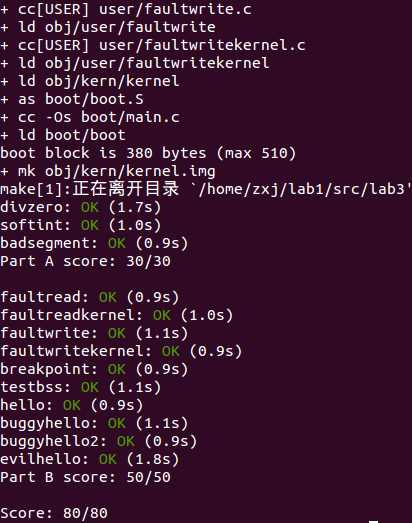
\includegraphics[width = .85\linewidth]{img/3.png}
        \caption{lab3实验结果-make grade}
        \label{fig::figure1}
    \end{figure}

\end{document}